\documentclass[10pt,a4paper]{paper}
%\documentclass[3p]{elsarticle}
%\documentclass[a4paper,reqno]{amsart}
\usepackage[british]{babel}
%\usepackage[garamond]{mathdesign}

\usepackage{amssymb,amsmath,graphicx,subfigure,float}
\usepackage{latexsym,caption,color,verbatim,enumerate,cancel}

\usepackage{authblk}

\usepackage{hyperref,url}

\usepackage{mathptmx}
%\usepackage{amsmath}
\usepackage{courier}
%\usepackage{amssymb}
%\usepackage{mathtools}
\usepackage{amsthm}
%\usepackage{enumerate}
\usepackage{enumitem,multicol}
\usepackage{tikz}
\usepackage{nicefrac}
\usepackage{bm}

\usepackage{mathtools}
%\usepackage{enumitem}
\usepackage{units}


\DeclareMathAlphabet\mathbfcal{OMS}{cmsy}{b}{n}

\theoremstyle{definition}
\newtheorem{vb}{Example}
\newtheorem{theorem}{Theorem}[section]
\newtheorem{prop}[theorem]{Proposition}
\newtheorem{corol}[theorem]{Corollary}
\newtheorem{lem}[theorem]{Lemma}
\newtheorem{defi}{Definition}
\newtheorem{proper}{Property}
\newtheorem{remark}{Remark}
\newtheorem*{remark*}{Remark}



\newcommand{\bpi}{\boldsymbol\pi}   
\newcommand{\vbpi}{\boldsymbol\pi}   
\newcommand{\vpi}{\scalebox{1.4}{\ensuremath\pi}} 

\newcommand{\ct}[1]{\tau_{#1}} 
\newcommand{\cn}[1]{\kappa_{#1}}  

\newcommand{\hyp}{\mathbf{h}} 
\newcommand{\ev}{\mathbf{e}}  

\newcommand{\hyps}{\mathbf{H}}
\newcommand{\evs}{\mathbf{E}}  

\newcommand{\restr}{_{|\cancel{\bf R}}} 
\newcommand{\giv}[1]{\big\vert_{#1}} 
\newcommand{\smallgiv}[1]{\vert_{#1}} 
\newcommand{\cd}{\!\cdot\!}  

\renewcommand{\arraystretch}{1.5}

\newcommand{\credal}{\mathcal{M}}
\newcommand{\newmid}{\hspace{0.9pt}\vert\hspace{0.9pt}}

\title{Exploiting Bayesian Network Sensitivity Functions for Inference in Credal Networks}


\renewcommand\Authfont{\flushleft\textsc}
\renewcommand\Affilfont{\normalfont\normalsize}
\setlength{\affilsep}{1em}


\author{\vspace{-10pt}~\\\normalfont Jasper De Bock\large\hfill\texttt{jasper.debock@ugent.be}}
\affil{Ghent University\\
 Department of Electronics and Information Systems\\
Technologiepark -- Zwijnaarde 914 \\
9052 Zwijnaarde \\ 
Belgium
\vspace{-5pt}
}
\author{\normalfont Janneke H. Bolt
\large\hfill\texttt{j.h.bolt@uu.nl}\\[8pt]
\Large\normalfont Silja Renooij
\large\hfill\texttt{s.renooij@uu.nl}}
\affil{Utrecht University\\
Department of Information and Computing Sciences\\Princetonplein 5, De Uithof \\
3584 CC Utrecht \\
The Netherlands
\vspace{10pt}
}

\begin{document}

\date{}
\maketitle


\begin{abstract}
A Bayesian network is a concise representation of a joint probability distribution, which can be used to compute any probability of interest for the represented distribution.  Credal networks were introduced to cope with the inevitable inaccuracies in the parametrisation of such a network. Where a Bayesian network is parametrised by defining unique local distributions, in a credal network sets of local distributions are given. From a credal network, lower and upper probabilities can be inferred. Such inference, however, is often problematic since it may require a number of Bayesian network computations exponential in the number of credal sets. In this paper we propose a preprocessing step that is able to reduce this complexity. We use sensitivity functions to show that for some classes of parameter in Bayesian networks the qualitative effect of a parameter change on an outcome probability of interest is independent of the exact numerical specification. We then argue that credal sets associated with such parameters can be replaced by a single distribution.
\end{abstract}

\section*{Todo's en opmerkingen}

\begin{itemize}
\item
Zoals eerder besproken heb ik de volgorde der auteurs aangepast. Mocht de huidige volgorde na het afwerken van de paper toch niet de respectievelijke hoeveelheden werk reflecteren, kan dat natuurlijk nog steeds aangepast worden. Naargelang de hoeveelheid input die er vanuit Lugano komt zullen er op het eind vermoedelijk ook nog (maximum) 2 extra namen bij komen.
\item
We hebben een nieuwe titel nodig
\item
Welk tijdschrift sturen we dit naar? Liever niet IJAR, want het begint er op te lijken dat ik daar nagenoeg alles naar toe stuur... JAIR is een optie, maar heeft het nadeel dat het Q2 is... {\color{red}Andere suggesties?}
\end{itemize}

\section{Introduction}\label{sec:introduction}
Ever since the introduction of Bayesian networks~\cite{Pearl:1988wk}, we have seen a growing interest for probabilistic graphical models in AI. A probabilistic graphical model concisely represents joint probability distributions over a set of stochastic variables, by combining the use of a graph to represent the independence relation among the variables with probability distributions over subsets of those variables. A \emph{Bayesian network} defines a unique joint probability distribution by combining an acyclic directed graph with local discrete distributions, one for each node in the graph conditioned on its parents. A Bayesian network can be used to infer any probability of interest from the represented distribution. 

Since in practice the specified probabilities, also called parameters, may be inaccurate, methods were developed to cope with such inaccuracies. A sensitivity analysis, for example, can be used to study the impact of inaccuracies on outcome probabilities of interest~\cite{Kjaerulff:2000ui}. Alternatively, \emph{credal networks} adopt the framework of imprecise probabilities~\cite{augustin2013:itip,Walley:1991vk} by allowing the use of closed convex sets of distributions (also called credal sets), rather than defining unique local distributions per variable. Credal networks as such represent a set of Bayesian networks~\cite{Antonucci:2014ty,Cozman:2000ug,Cozman:2005ct}. 

One of the main computational problems in a credal network is the computation of tight lower and upper bounds on the outcome probabilities that correspond to the represented Bayesian networks. These computations in essence require a number of Bayesian network inferences that is exponential in the number of imprecise local credal sets, which are the local credal sets that consist of more than one distribution. 

Although this combinatoric explosion can, in general, not be avoided, in many cases a reduction is possible. For example, similar to what can be done for Bayesian networks, it is possible to apply a preprocessing step in which the variables that are irrelevant for a specific problem, such as d-separated or barren nodes, are pruned in advance~\cite{Cozman:2000ug}. In this paper, we introduce a second type of preprocessing step to reduce the combinatoric complexity of credal network inference. Unlike the use of d-separation or the removal of barren nodes, our preprocessing step is tailored specifically to credal networks, and does not apply to Bayesian networks, as it involves replacing some of the local imprecise credal sets by a single distribution.

{\color{red} *** It would be good to add a simple example already here, where we show a very simple network and illustrate what we do ***}

In order to prove the validity of our preprocessing step for credal network inference, we exploit results that we derive from Bayesian network sensitivity functions. More specifically, we use sensitivity functions to prove that for certain categories of distributions we can predict the qualitative effect of changing their parameters on an outcome probability, irrespective of the numerical specification of the network. In a credal network, this result allows us to identify, prior to the inference, local credal sets that can be replaced by a single distribution without changing the result of the inference.
By applying this preprocessing step, the number of imprecise local credal sets and the corresponding combinatoric complexity of inference is reduced. 
Moreover, we demonstrate that for some widely used special classes of networks
even all credal sets can be replaced by a single distribution, thereby essentially reducing the problem of computing a lower or upper probability in a credal network to an inference problem in a single Bayesian network.

This paper is organised as follows. In Section~\ref{sec:notation}, we introduce the notation used throughout the paper. In Section~\ref{sec:bayesian}, we start with a brief review of Bayesian networks and subsequently derive the properties of sensitivity functions for Bayesian networks that we want to exploit in the context of credal networks. Section~\ref{sec:credal} introduces the concept of a credal network, and then uses the results in Section~\ref{sec:bayesian} to establish the aforementioned preprocessing technique. We end the paper with conclusions and suggestions for future research.


\section{Notation}\label{sec:notation}
This paper is concerned with graphical models for (sets of) joint probability distributions $\Pr({\bf V})$ over a set of finite-valued random variables~${\bf V}$.

We use upper case $V$ to denote a single random variable, writing $v \in V$ to indicate a value (lowercase $v$) of $V$. For binary-valued $V$, we use $v$ and $\overline{v}$ to denote its two possible value assignments.
Boldfaced letters are used to indicate sets (capitals), both of variables and of value assignments, or a joint value assignment (lowercase) to a set of variables; the distinction will be clear from the context. For example $V \in {\bf W}$ indicates that $V$ is a variable in a set of variables ${\bf W}$, whereas ${\bf w}\in {\bf W}$ indicates that ${\bf w}$ is a joint value assignment of that same set of variables~${\bf W}$. 

Two value assignments are said to be compatible, denoted by $\sim$, if they agree on the values of the shared variables; otherwise they are said to be incompatible, denoted by $\nsim$. For example, for three distinct variables $U$, $V$ and $W$ in ${\bf V}$, and value assignments $u,u'\in U$, $v\in V$ and $w\in W$ such that $u\neq u'$, we have that $u v \sim u v w$ and $u v \nsim u' v w$. Assignments to disjoint sets are always considered to be compatible.

The probabilistic graphical models that we consider are Bayesian networks and credal networks. The graphical part of these models consists of a directed graph, the nodes of which have a one-to-one correspondence with the random variables $V$ in ${\bf V}$. For a given node $V$, $\vpi$ indicates its set of parents in the directed graph, and we will use $\vbpi$ 
to indicate a joint instantiation of these parents. %\anote{Het volgende er dus uit: Both types of networks associate a (set of) local probability distribution(s) $\Pr(V \newmid \vbpi)$ with each node in the graph and each parent instantiation.}
Without loss of generality, we assume that the set ${\bf V}$ of all random variables consists of  %\anote{
the disjoint subsets  $\hyps$ (hypothesis variables), $\evs$ (evidence variables) and  ${\bf R}$, with ${\bf V} = \hyps \cup \evs \cup {\bf R}$. %} \anote{ Het volgende er dus ook uit: We are interested in computing (bounds on) probabilities of the form $\Pr(\hyp \newmid \ev)$ for hypothesis variables $\hyps$ and evidence variables $\evs$.} 
The sets of hypothesis variables and evidence variables that do not have parents in ${\bf R}$ are denoted by $\hyps\restr$ and $\evs\restr$, respectively. Similarly, the set $\hyps_{|\cancel{\bf H}}$ consists of those hypothesis variables that have no parents in ${\bf H}$. 

Finally, when referring to monotonic functions, we will use the term \emph{increasing} to indicate both strictly increasing and non-decreasing functions; likewise \emph{decreasing} refers to both strictly decreasing and non-increasing functions.


\section{Bayesian Network's Sensitivity Properties}\label{sec:bayesian}
In this section, we first briefly review Bayesian networks and sensitivity analysis. Subsequently, we establish guarantees on the behaviour of sensitivity functions for some categories of parameters. Next, we use these results to define types of local distributions, which will then allow us in Section~\ref{sec:credal} to exploit our results in the context of credal networks.

\subsection{Bayesian network preliminaries}\label{sec:bayesian:prelim}
A Bayesian network ${\mathcal B}$ is a concise representation of a joint probability distribution. It uses a directed acyclic graph to capture the (in)dependences among its variables ${\bf V}$ using the well-known d-separation criterion \cite{Pearl:1988wk}.\footnote{For any three disjoint sets of
nodes $X$, $Y$, $Z$, the set $Z$ is said to d-separate $X$ and $Y$ if there do not exist any active chains between $X$ and $Y$ given evidence for $Z$. A chain between two nodes is active if each of its head-to-head nodes is either instantiated or has an instantiated descendant, and none of its other nodes are instantiated. The variables captured by d-separated nodes are considered probabilistically independent.}  Furthermore, for each variable $V\in{\bf V}$, it specifies exactly one local distribution $\Pr(V\newmid \vbpi)$ over the values of $V$ for each value assignment $\vbpi$ to $\vpi$;  the separate probabilities in these distributions are termed the network's \emph{parameters}. The joint probability distribution $\Pr$ factorises over the local distributions as follows:
\begin{equation*}
\Pr({\bf v})=\prod_{V \in {\bf V}}\Pr(v\newmid \vbpi)\giv{v\vbpi\sim {\bf v}}
\end{equation*}
where the notation $\smallgiv{\mbox{\footnotesize prop}}$ is used to indicate the properties the arguments in the preceding formula adhere to. Outcome probabilities of the form $\Pr(\hyp\newmid\ev)$ can be computed with various algorithms~\cite{Jensen:2007fb}. 

An example Bayesian network is shown in Figure~\ref{fig-vbMAP-TC}. The figure shows a graph with hypothesis variables $\hyps = \{G,H,K\}$ (double circles), evidence variables $\evs= \{E,F\}$ (shaded), and remaining variable ${\bf R} = \{R\}$. 
The figure also shows conditional probability tables (CPTs) that specify the local distributions. Actual numbers are not provided, but the top row in the table for $\Pr(H\newmid G)$ could for example specify the parameters $\Pr(h\newmid g)=0.4$ and $\Pr(\overline{h}\newmid g)=0.6$. 

The probabilities computed from a Bayesian network depend on the parameters specified in the network, which are inevitably inaccurate. To study the effects of such inaccuracies on an output probability of interest, a sensitivity analysis can be performed. One approach to performing a sensitivity analysis is to compute so-called sensitivity functions~\cite{Kjaerulff:2000ui}. 
An $n$-way sensitivity function describes an output probability of interest $\Pr(\hyp\newmid \ev)$ as a function of $n$ network parameters $\vec{x}=\{x_1,\ldots ,x_n\}$:
\begin{equation*}
\Pr(\hyp\newmid \ev)(\vec{x}) = \frac{\Pr(\hyp\ev)(\vec{x})}{\Pr(\ev)(\vec{x})}
\end{equation*}
where both the numerator and the denominator are known to be multi-linear expressions in $\vec{x}$. For $n=1$, the one-way sensitivity function takes the general form
\begin{equation*} 
\Pr(\hyp\newmid \ev)(x) = \frac{\ct{1}\cdot x+\ct{2}}{\cn{1}\cdot x+\cn{2}}
\end{equation*}
where the constants $\ct{1},\ct{2},\cn{1}$ and $\cn{2}$ are composed of non-varied network parameters. Throughout this paper we assume  $\Pr(\ev)$ to be, and to remain, strictly positive.

Upon varying a parameter $x$ of a distribution, the other parameters of the same distribution have to be co-varied to let the distribution sum to $1$. If the distribution is associated with a binary variable, the co-varying parameter equals $1-x$. If a variable is multi-valued, however, different co-variation schemes are possible~\cite{renooij20141022}.

\subsection{Parameters that have no effect on the inference}

{\color{red}*** I added an extra subsection here, and have copied a bit of text that used to belong to the previous section. My suggestion would be to, in this section, characterise all the parameters that have no effect on the inference. At first sight, I think these will be parameters that belong to d-separated nodes and barren nodes, and (partially overlapping) parameters of Type 0. ***}

Based upon graphical considerations alone, in computing a probability $\Pr(\hyp\newmid\ev)$, and thus also for performing sensitivity analyses with respect to this output probability, a Bayesian network can be safely pruned by removing variables that are either d-separated from $\hyps$ given $\evs$, or that are barren given these sets.\footnote{Barren variables are in the set $\bf{R}$ and have just barren descendants.}
The remaining variables all have evidence or parameters that may be required for the computation of $\Pr(\hyp\newmid\ev)$~\cite{shachter98a}. This set of requisite variables coincides with the union of $\evs$ and the so-called sensitivity set~\cite{Meekes2015}, which is the set of variables for which a change in one of its parameters may result in a change in $\Pr(\hyp\newmid\ev)$~\cite{Coupe2002}. In our example network in Figure~\ref{fig-vbMAP-TC} all variables are in the sensitivity set of $\Pr(ghk\newmid ef)$.


\begin{figure*}[t]
\begin{center}
%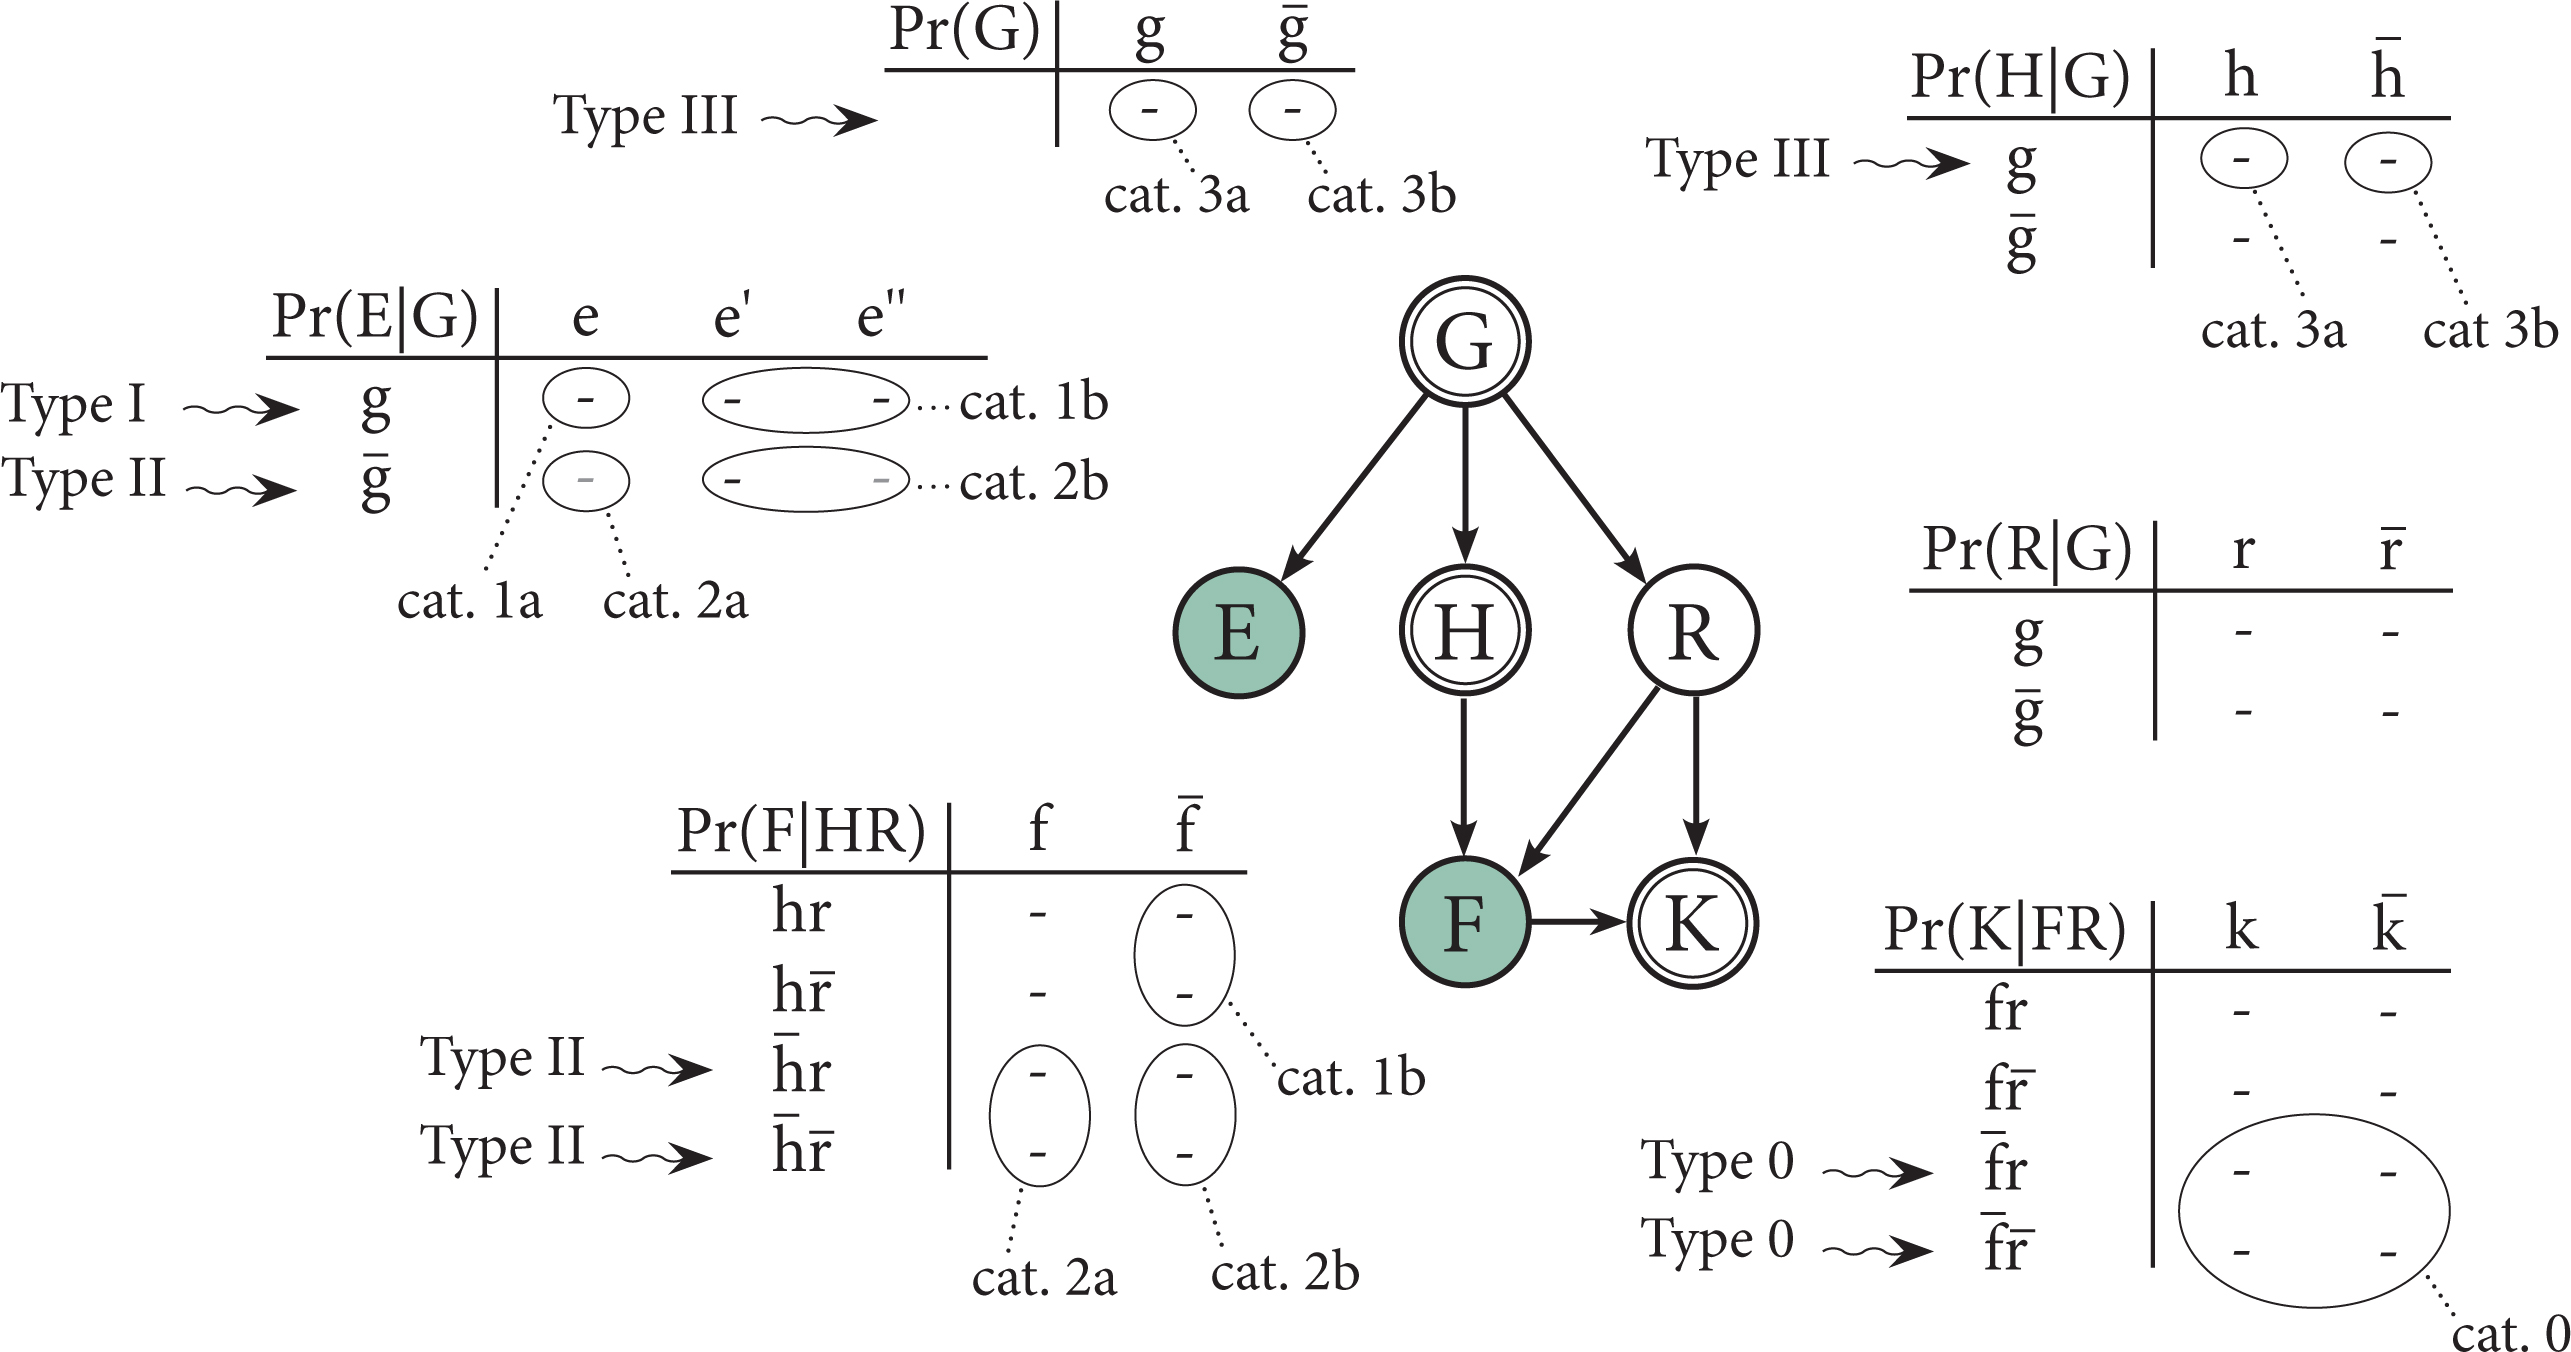
\includegraphics[width=0.75\textwidth]{fig-vbMAP-TC2.jpg}
\begin{tikzpicture}
      \node[anchor=south west,inner sep=0] (plot) at (0,0) {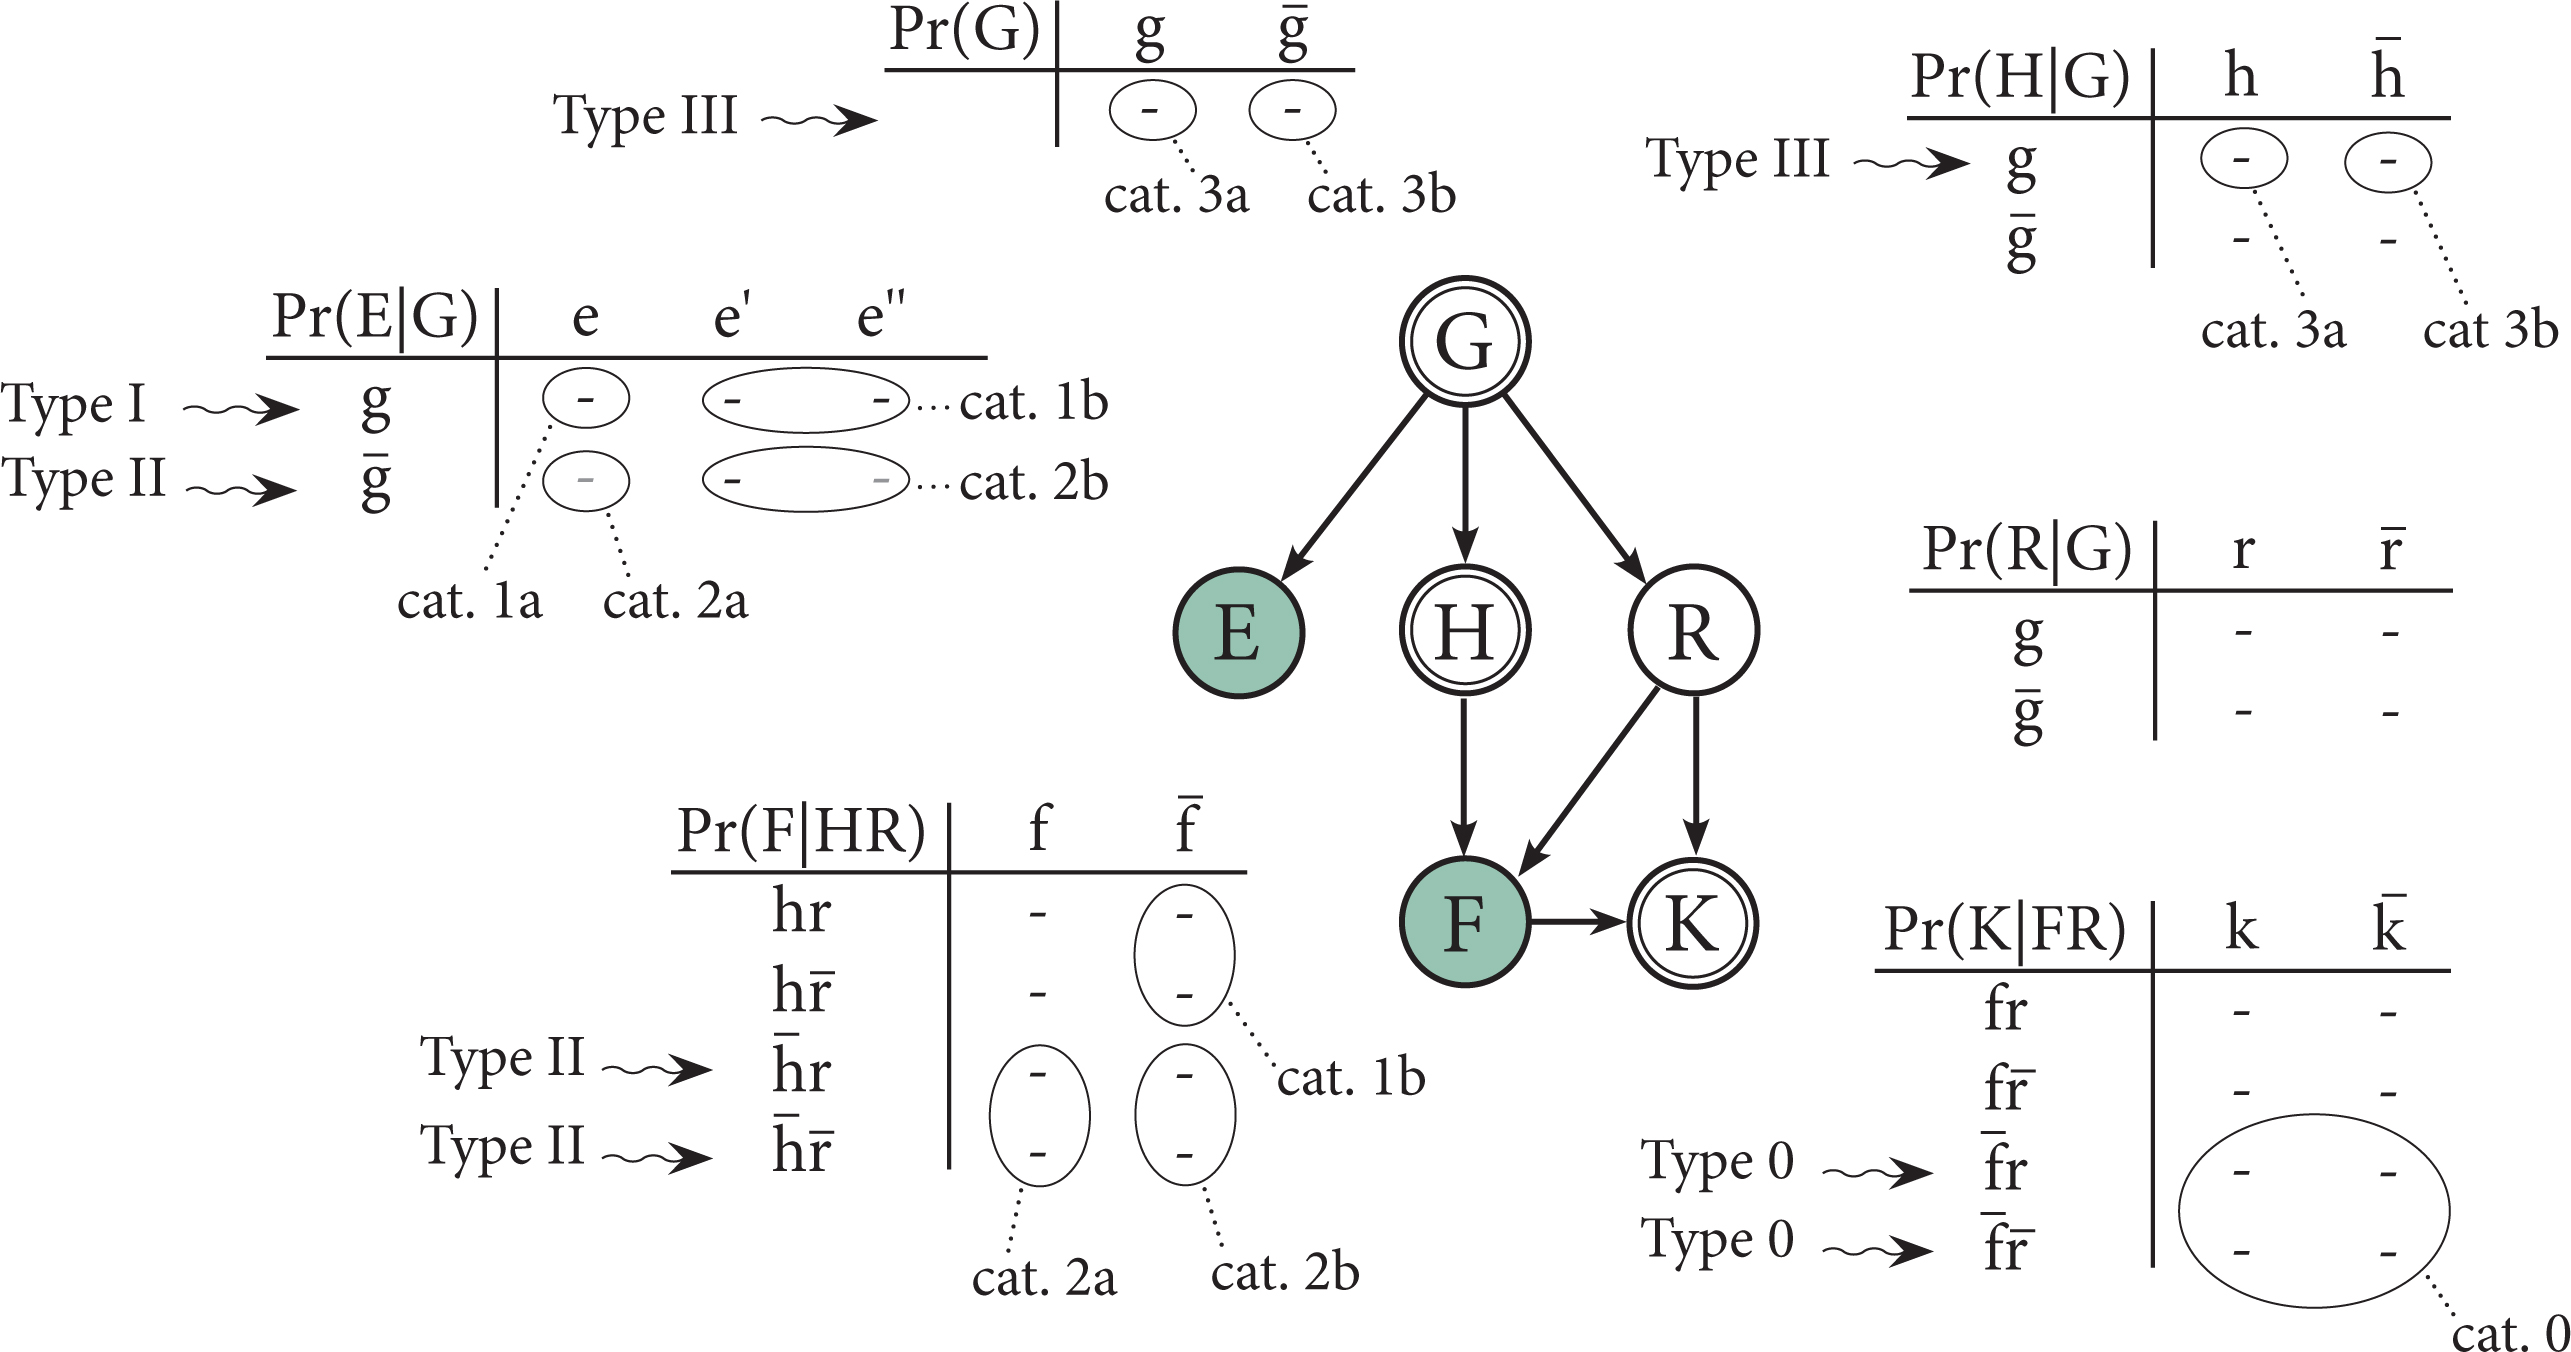
\includegraphics[width=106mm]{fig-vbMAP-TC2}};
      \begin{scope}[x={(plot.south east)},y={(plot.north west)}]
        \node[below, align=left, fill=black!20] at (0.5,0.6) {\color{red}I want to turn this into a tikz picture.\\ \color{red}This will allow us to easily create extra ones,\\ \color{red}
        and to use notation that is uniform with the main text};
      \end{scope}
\end{tikzpicture}
\vspace{12pt}
\caption{An example Bayesian---and credal---network. The CPTs are labelled with parameter categories (see Table~\ref{cat}) and distribution types (see Section~\ref{sec:bayesian:distributiontypes}) with respect to output probability $\Pr(ghk\newmid ef)$.}
\label{fig-vbMAP-TC}
\end{center}
\end{figure*}

\subsection{Parameters with a guaranteed monotone effect}\label{sec:bayesian:guaranteedeffects}

{\color{red}*** I would suggest that in this section, we focus mostly on parameters that do not belong to the categories in the previous section. Perhaps we can even assume that d-separated and barren nodes have already been removed, and that evidence absorbtion has already been applied? ***}

In this section, we first consider one-way sensitivity functions $\Pr(\hyp \newmid \ev)(x)$ and identify categories of parameters that are guaranteed to give monotonically increasing and parameters that are guaranteed to give monotonically decreasing one-way functions. 
We also identify parameters inside the sensitivity set of $\Pr(\hyp \newmid \ev)$ that are not used in computing the outcome probability $\Pr(\hyp \newmid \ev)$. 
Next, we use these results to provide guarantees on $n$-way functions $\Pr(\hyp \newmid \ev)(\vec{x})$. 

We begin by categorising the different parameters $x=\Pr(v\newmid \bpi)$ of a Bayesian network with respect to a specific outcome probability $\Pr(\hyp\newmid\ev)$. We only categorise the subset of all parameters for which we can provide guarantees on their qualitative effect on the outcome probability. The categorisation is given in Table \ref{cat}. For our example network in Figure \ref{fig-vbMAP-TC}, the categories are indicated with respect to the output probability \mbox{$\Pr(ghk\newmid ef)$}. 


\begin{table}
\begin{center}
\caption{Categorisation of parameters $x=\Pr(v\newmid \bpi)$ with respect to the outcome probability $\Pr(\hyp\newmid\ev)$.}
\vspace{8pt}
\begin{tabular}{r||c|c}
& $\bpi \sim \hyp$ & $\bpi\nsim \hyp$\\
\hline\hline
$\bpi\nsim \ev$ & cat. 0 & cat. 0\\
\hline
$V \in\evs$, $v\nsim \ev$ and $\bpi\sim \ev$& cat. 1b & cat. 2b\\
\hline
$V\in\evs\restr$~~and $v\,\bpi \sim \ev$ & cat. 1a & cat. 2a\\
\hline
$V \in\evs\setminus\evs\restr$~~and $v\,\bpi \sim \ev$ & - & cat. 2a\\
\hline
binary $V \in\hyps\restr$~~and $\bpi \sim \ev$ & cat. 3a ($v\sim \hyp$) & -\\
 & cat. 3b ($v\nsim \hyp$) & 
\label{cat}
\end{tabular}
\end{center}
\end{table}

The following proposition states that parameters from category~1a result in sensitivity functions that are monotonically increasing, whereas parameters from category~2a give monotonically decreasing sensitivity functions, \emph{irrespective of the values of the non-varied network parameters and irrespective of the co-variation scheme that is used.}  

\begin{prop}\label{mono1}
Consider a Bayesian network ${\mathcal B}$ and a probability of interest $\Pr(\hyp\newmid \ev)$. Let $x=\Pr(v\newmid \bpi)$ be a parameter of\/ $V\in\evs$ with $v\,\bpi\sim\ev$. 
If\/ $V\in\evs\restr$~~and $\bpi\sim\hyp$, then the sensitivity function $\Pr(\hyp\newmid \ev)(x)$ is monotonically increasing. If\/ $\bpi\nsim\hyp$, then the sensitivity function 
$\Pr(\hyp\newmid \ev)(x)$ is monotonically decreasing. 
\end{prop}

\noindent {\bf Proof.} 
We first consider the numerator of the sensitivity function:
\begin{equation}\label{eq:numerator}
\Pr(\hyp\ev)= \sum_{{\bf r}\in{\bf R}}\Pr({\bf r}\hyp\ev) = 
\sum_{{\bf r}\in{\bf R}} \prod_{V^*\in {\bf V}} \Pr(v^* \newmid \vbpi^*)\giv{v^*\vbpi^*\sim {\bf r}\hyp\ev}
\end{equation} 
Note that $x=\Pr(v\newmid \bpi)$ is a factor in this expression only if $\bpi \sim \hyp$. For $\bpi \nsim \hyp$, therefore, $\Pr(\hyp\ev)(x) = \ct{1}$ for some constant $\ct{1} \geq 0$. 
%
Returning to the case where $\bpi \sim \hyp$, we observe that if $V\in\evs\restr$, we  have that $\bpi\sim {\bf r}\hyp\ev$ for all ${{\bf r}\in{\bf R}}$ and we thus find that
\vspace{4pt}
\begin{equation*}
\Pr(\hyp\ev)(x)= x\cdot 
\Bigl(
\sum_{{\bf r}\in{\bf R}} \prod_{V^*\in {\bf V}\setminus\{V\}} \Pr(v^* \newmid \vbpi^*)\giv{v^*\vbpi^*\sim {\bf r}\hyp\ev} 
\Bigr)
\end{equation*}
Given $\bpi\sim\hyp$ and $V \in \evs\restr$, therefore, $\Pr(\hyp\ev)(x) = x\cdot\ct{1}$ for some constant $\ct{1} \geq 0$. 

Next, we consider the denominator of the sensitivity function:
\begin{align}
\Pr(\ev)&=\sum_{{\bf r}\in{\bf R},{{\bf h^*}\in{\bf H}}}\Pr({\bf r}\hyp^*\ev)
=\sum_{{\bf r}\in{\bf R},{{\bf h^*}\in{\bf H}}} \prod_{V^*\in {\bf V}} \Pr(v^*\newmid \vbpi^*)\giv{v^*\vbpi^*\sim {\bf r}\hyp^*\ev}\label{eq:denominator}
\end{align}
We observe that $x=\Pr(v\newmid \bpi)$ is a factor in each term of the summation for which $\bpi\sim{\bf r}\hyp^*$, and otherwise is absent. That is, no term includes $x$ as a co-varying parameter. Therefore, $\Pr(\ev)(x) = \cn{1}\cdot x + \cn{2}$, for constants $\cn{1},\cn{2} \geq 0$.  

We are now able to determine the general form of the sensitivity function $\Pr(\hyp\newmid\ev)(x)$ under the given conditions.
Moreover, we can use the first derivative of this sensitivity function to determine whether the function is increasing or decreasing.
If $\bpi\sim\hyp $ and $V \in \evs\restr$, we find that
\begin{equation*}
\Pr(\hyp\newmid\ev)'(x)=\frac{\ct{1}\cdot \cn{2}}{(\cn{1}\cdot x+\cn{2})^2}.
\end{equation*}
This first derivative is always non-negative which implies that $\Pr(\hyp\newmid \ev)(x)$ is a monotone increasing function, irrespective of the values of the non-varied network parameters and irrespective of the co-variation scheme. 
If $\bpi\nsim\hyp$, we find that
\begin{equation*}
\Pr(\hyp\newmid\ev)'(x)=\frac{-\ct{1}\cdot \cn{1}}{(\cn{1}\cdot x+\cn{2})^2}.
\end{equation*}
This first derivative is always non-positive, which implies that $\Pr(\hyp\newmid \ev)(x)$ is a monotone decreasing function, irrespective of the values of the non-varied network parameters and irrespective of the co-variation scheme. 
\hfill $\Box$

\bigskip

Our next proposition states that parameters from category 3a result in monotonically increasing sensitivity functions, whereas parameters from category 3b give monotonically decreasing sensitivity functions, again \emph{irrespective of the values of the non-varied network parameters.}  The proposition concerns parameters for binary hypothesis variables, which implies that the co-variation scheme is fixed. 

\begin{prop}\label{mono2}
Consider a Bayesian network ${\mathcal B}$ 
and a probability of interest $\Pr(\hyp\newmid \ev)$. 
Let $x=\Pr(v\newmid \bpi)$ be a parameter of a binary variable $V\in\hyps\restr$~, with $\bpi\sim\ev$ and $\bpi\sim\hyp$. If\/ $v\sim\hyp$ then the sensitivity function $\Pr(\hyp\newmid \ev)(x)$ is monotonically increasing. If\/ $v\nsim\hyp$ then 
$\Pr(\hyp\newmid \ev)(x)$ is monotonically decreasing.
\end{prop}

\noindent {\bf Proof.} 
We first consider the parameters $x$ with $v\sim \hyp$.
As in the proof of Proposition~\ref{mono1}, the numerator of the sensitivity function can be rewritten as
\[\Pr(\hyp\ev)(x)= x\cdot 
\Bigl(
\sum_{{\bf r}\in{\bf R}} \prod_{V^*\in {\bf V}\setminus\{H\}} \Pr(v^* \newmid \vbpi^*)\giv{v^*\vbpi^*\sim {\bf r}\hyp\ev} 
\Bigr)
\]
because, under the given conditions, $x$ is a factor in all terms of the summation. Therefore, we have that $\Pr(\hyp\ev)(x) = x\cd\ct{1}$, for some constant $\ct{1} \geq 0$. 

The assumption that $V$ is binary enforces the following co-variation scheme:  $\Pr(\overline{v}\newmid{\bpi})=1-\Pr(v\newmid\bpi)$. Therefore, with respect to the denominator of the sensitivity function---see Equation~\eqref{eq:denominator}--- 
we observe the following: 1) $x$ itself is a factor in any term of the summation for which $\bpi\sim \hyp^*$ and $v\sim \hyp^*$, 2) $x$ appears as $(1-x)$ for $\bpi\sim \hyp^*$ and $v\nsim \hyp^*$, and 3) $x$ is absent whenever $\bpi\nsim\hyp^*$. Hence, $\Pr(\ev)(x) = x\cd\cn{1}+(1-x)\cd\cn{2}+\cn{3}$, with constants $\cn{i}\geq 0$, $i=1,2,3$. 

We now find that the first derivative of the sensitivity function equals 
the following non-negative function:
\[
\Pr(\hyp\newmid\ev)'(x)=\frac{(\cn{2}+\cn{3})\cd\ct{1}}{(\cn{2}+\cn{3}+\cn{1}\cd x-\cn{2}\cd x)^2}
\]
This implies that $\Pr(\hyp\newmid \ev)(x)$ is a monotonically increasing function irrespective of the values of the non-varied network parameters. 

Next, we consider the parameters $x= \Pr(v\newmid\bpi)$ with $v\nsim \hyp$. Since we know that $\Pr(v\newmid{\bpi})=1-\Pr(\overline{v}\newmid\bpi)$ with $\overline{v}\sim\hyp$, an increase (decrease) of $x$ is equivalent to a decrease (increase) of the parameter consistent with $\hyp$. 
Hence, using the first part of this proof, it follows that $\Pr(\hyp\newmid \ev)(x)$ is a monotonically decreasing function irrespective of the values of the non-varied network parameters. \hfill $\Box$

\bigskip

Although the above propositions are concerned with one-way sensitivity functions, we have shown that their monotone increasing or decreasing behaviour does not depend on the actual values of the non-varied parameters which determine the constants of the function. As a result, our observations extend to specific $n$-way sensitivity functions.

\begin{theorem}
Consider a Bayesian network ${\mathcal B}$ and a probability of interest $\Pr(\hyp\newmid\ev)$. 
Let ${\vec{x}}_+=\{x_1^+,\ldots ,x_k^+\}$ be a set of parameters from categories 1a and/or 3a, and let ${\vec{x}}_-=\{x_1^-,\ldots ,x_l^-\}$ be a set of parameters from categories 2a and/or 3b. Then the $(k+l)$-way sensitivity function $\Pr(\hyp\newmid\ev)({\vec{x}}_+,{\vec{x}}_-)$ is monotonically increasing for increasing parameters $x_i^+$ and decreasing parameters $x_i^-$; 
the sensitivity function is monotonically decreasing for decreasing $x_i^+$ and increasing $x_i^-$. 
\label{theo}
\end{theorem}

\noindent {\bf Proof.} 
From Propositions \ref{mono1} and \ref{mono2} we have that a one-way sensitivity function $\Pr(\hyp\newmid\ev)(x_i^+)$ increases with increasing $x_i^+$ and a one-way sensitivity function $\Pr(\hyp\newmid\ev)(x_i^-)$ increases with decreasing $x_i^-$, irrespective of the values of the non-varied parameters, and irrespective of the co-variation scheme. Given a simultaneous increase of parameters in $\vec{x}_+$ and decrease of parameters in $\vec{x}_-$, therefore, the probability $\Pr(\hyp\newmid\ev)(\vec{x}_+,\vec{x}_-)$ will increase. A similar observation holds for decreasing $x_i^+$ and increasing $x_i^-$. 
\hfill $\Box$

\bigskip

The above results describe an output probability of interest as a function of changing input parameters of categories 1a, 2a, 3a and 3b. The example network in Figure~\ref{fig-vbMAP-TC} also includes parameters of category 0, 1b and 2b. 
Parameters of these categories are not used in computing the output probability.
For category 0, the parameters make up an entire local distribution (see e.g. the CPT for $\Pr(K \newmid FR)$); for parameters of categories 1b and 2b, parameters are in a local distribution with a parameter of category 1a or 2a (see e.g. the CPTs for $\Pr(E\newmid G)$ and $\Pr(F\newmid HR)$). 

\begin{prop}\label{constant}
Consider a Bayesian network ${\mathcal B}$ and a probability of interest $\Pr(\hyp\newmid \ev)$. Let $\Pr(v\newmid \bpi)$ be a parameter. If\/ $v\nsim\ev$ and/or $\bpi\nsim\ev$, then $\Pr(v\newmid \bpi)$ is not used in the computation of\/ $\Pr(\hyp\newmid \ev)$. 
\end{prop}
\noindent {\bf Proof.} 
As before, we have that 
\[\Pr(\hyp\newmid \ev) = \frac{\Pr(\hyp\ev)}{\Pr(\ev)}\]
with numerator
\[\Pr(\hyp\ev)= \sum_{{\bf r}\in{\bf R}}\Pr({\bf r}\hyp\ev) = 
\sum_{{\bf r}\in{\bf R}} \prod_{V^*\in {\bf V}} \Pr(v^* \newmid \vbpi^*)\giv{v^*\vbpi^*\sim {\bf r}\hyp\ev} 
\]
The parameter $\Pr(v\newmid \bpi)$ can only be a factor in this numerator if $v\sim\ev$ and $\bpi\sim\ev$. 
A completely analogous observation holds for the denominator as well. \hfill $\Box$
 
\bigskip
Note that we cannot conclude from the above proposition that the sensitivity function $\Pr(\hyp\newmid \ev)(x)$ for parameters $x=\Pr(v\newmid \bpi)$ of categories 1b and 2b is constant. A change of such parameters may, by co-variation, induce a change in the parameter $\Pr(v'\newmid \bpi)$ of the same local distribution with $v'\sim\ev$ which \emph{is} used in the computation of $\Pr(\hyp\newmid \ev)$. The actual value of a parameter with $v\nsim\ev$, however, is irrelevant for $\Pr(\hyp\newmid \ev)$. 
We {\em can} conclude that the sensitivity function $\Pr(\hyp\newmid\ev)(x)$ for parameters of category 0 is a constant, however, since given a parameter with $\bpi\nsim\ev$ this condition is fulfilled for all parameters in the same local distribution. 

\subsection{Defining local distribution types\label{sec:bayesian:distributiontypes}}
{\color{red}*** I don't really know what to do with this section. Perhaps we can extend the distributions of Type 0 to include d-separated and barren ones... or perhaps we assume that those have already been removed?}


In the previous subsection we have focused on properties of different categories of parameters in a Bayesian network. In order to apply our results in the context of credal networks, it will be useful to lift these properties to the level of distributions. To this end, 
we define four types of local distributions $\Pr(V\newmid\vbpi)$, again with respect to a specific outcome probability of interest $\Pr(\hyp\newmid\ev)$.

\begin{defi}[Local distribution of Type 0]\label{def:local:type0}
Consider a Bayesian network ${\mathcal B}$ and a probability of interest $\Pr(\hyp\newmid\ev)$.  A local distribution $\Pr(V\newmid \vbpi)$ is said to be of\, \emph{Type 0} if $\vbpi\nsim\ev$.
\end{defi}
All parameters of a local distribution of Type 0 are in category 0. From Proposition~\ref{constant}, we know that parameters from a local distribution of Type 0 are irrelevant for the computation of the outcome probability $\Pr(\hyp\newmid\ev)$. 

\begin{defi}[Local distribution of Type I]\label{def:local:type1}
Consider a Bayesian network ${\mathcal B}$ and a probability of interest $\Pr(\hyp\newmid\ev)$. A local distribution $\Pr(V\newmid \vbpi)$ is said to be of\, \emph{Type I} if\/ $\vbpi\sim\ev$, $V\in \evs\restr$ and $\vbpi\sim\hyp$.
\end{defi}
The unique parameter of a distribution of Type I with $v\sim\ev$ is in category 1a. Any other parameter $\Pr(v'\newmid\ev)$ of the distribution is in category 1b and is therefore irrelevant for computing $\Pr(\hyp\newmid\ev)$, since $v'\nsim\ev$.
Given changes in a local distribution of Type I, therefore, knowing the qualitative change of the parameter with $v\sim\ev$ suffices to know the qualitative effect of the changes in the entire distribution on $\Pr(\hyp\newmid\ev)$. In particular, an increase (decrease) of this parameter results in an increase (decrease) of $\Pr(\hyp\newmid\ev)$.

\begin{defi}[Local distribution of Type II]\label{def:local:type2}
Consider a Bayesian network ${\mathcal B}$ and a probability of interest $\Pr(\hyp\newmid\ev)$. A local distribution $\Pr(V\newmid \vbpi)$ is said to be of\, \emph{Type II} if\/ $\vbpi\sim\ev$, $V\in \evs$ and $\vbpi\nsim\hyp$.
\end{defi}
Analogous to distributions of Type I, knowing the qualitative change of the parameter with $v\sim\ev$ is sufficient to know the qualitative effect of changes in the entire local distribution on $\Pr(\hyp\newmid\ev)$. Now the unique parameter with $v\sim\ev$ is in category 2a, which implies that an increase (decrease) of this parameter results in an decrease (increase) of $\Pr(\hyp\newmid\ev)$. 

\begin{defi}[Local distribution of Type III]\label{def:local:type4}
Consider a Bayesian network ${\mathcal B}$ and a probability of interest $\Pr(\hyp\newmid\ev)$. A local distribution $\Pr(V\newmid \vbpi)$ is said to be of\, \emph{Type III} if\/ $\vbpi\sim\ev$, $\vbpi\sim\hyp$, $V\in \hyps\restr$ and $\vert V\vert =2$.
\end{defi}
Distributions of Type III consist of exactly two parameters, one for $v$ and one for $\overline{v}$, which are related by the fixed co-variation scheme: $\Pr(v\newmid{\bpi})=1-\Pr(\overline{v}\newmid\bpi)$. The parameter that is compatible with $\hyp$ is in category 3a, which implies that an increase (decrease) of this parameter results in an increase (decrease) of $\Pr(\hyp\newmid\ev)$. The parameter that is not compatible with $\hyp$ is in category 3b, which implies that the concurrent decrease (increase) of this parameter results in an increase (decrease) of $\Pr(\hyp\newmid\ev)$ as well.

\bigskip
By Theorem \ref{theo} and Proposition \ref{constant} we have that, given simultaneous changes in multiple local distributions, $\Pr(\hyp\newmid\ev)$ will increase (decrease) given an increase (decrease) of the parameters with $v\sim\ev$ in the distributions of Type I and III and a decrease (increase) of the parameters compatible with $v\sim\ev$ in the distributions of Type II. The outcome probability $\Pr(\hyp\newmid\ev)$ is not affected by changes in local distributions of Type 0. 

\subsection{Important special cases}\label{sec:bayesian:specialcase}
In Section~\ref{sec:bayesian:distributiontypes} we identified types of distributions for which we can guarantee the direction of change in $\Pr(\hyp\newmid\ev)$ upon changes in certain parameters from those distributions. In general, as illustrated in Figure~\ref{fig-vbMAP-TC}, a network will include distributions that do not belong to any of those types. We can, however, identify classes of networks for which the majority of distributions---or even all of them---can be classified as Type 0, I, II or III.

Consider for example a network obeying the following constraint: each observed variable only has hypothesis variables or other observed variables as parents, that is, $\evs=\evs\restr$.
It then follows from Definitions~\ref{def:local:type0}--\ref{def:local:type2} that all local distributions of the observed variables are of type 0, I or II. Bayesian network classifiers with full evidence obey this constraint. Bayesian classifiers, a special type of Bayesian network, are widely used in practice (see~\cite{Flores2012} for an overview).

Now consider a network obeying the constraint that all hypothesis variables are binary valued and can only have observed variables as parents, that is, $\hyps=\hyps_{|\cancel{\bf R}}\cap\hyps_{|\cancel{\bf H}}$ and $|V|=2$ for each $V$ in $\hyps$. It then follows from Definitions~\ref{def:local:type0} and~\ref{def:local:type4} that all local distributions of the hypothesis variables are of Type 0 or III.\footnote{$V\in\hyps_{|\cancel{\bf H}}$ implies that $\bpi\sim\hyp$} This second constraint is for example obeyed by Bayesian network classifiers with a single binary class variable, or by Bayesian network classifiers with multiple binary class variables, provided that these class variables have no class parents.\footnote{Note that, by definition, in Bayesian classifiers class variables do not have feature parents, as a consequence, $\hyps=\hyps_{|\cancel{\bf R}}$, even in case of incomplete evidence.} Given full evidence, these two types of Bayesian network classifiers also satisfy the first constraint, it follows therefore that, given full evidence, for those networks all the distributions are of Type 0, I, II or III.


\section{An Application to Credal Networks}\label{sec:credal}

Since a sensitivity function is an object that is associated with a given Bayesian network, it might at first sight seem as if it has little to do with credal networks, because these are essentially sets of Bayesian networks. However, for the particular sensitivity properties that we developed in the previous section, this is not the case. As we will explain in this section, these sensitivity properties allow us to replace some of the local credal sets of a credal network by a single probability mass function, and in this way, the combinatoric nature of credal network inference can be reduced.


\subsection{Credal network preliminaries}\label{sec:credal:prelim}

An important limitation of Bayesian networks is that they require the exact specification of a large number of probabilities. Since these probabilities have to be elicited from experts or estimated from data, this requirement is often unrealistic. By enforcing it anyway, as is conventionally done, we run the risk  of ending up with a model whose precision is unwarranted, thereby making the resulting conclusions unreliable. In order to avoid these issues, credal networks explicitly drop the assumption that probabilities should be specified exactly, and instead adopt the framework of imprecise probabilities~\cite{augustin2013:itip,Walley:1991vk,Walley:2000ef}, thereby trading off precision for reliability.  

Basically, a \emph{credal network}~\cite{Antonucci:2014ty,Cozman:2000ug,Cozman:2005ct} is just a Bayesian network of which the local models are partially specified, in the sense that they are only known to belong to some set of candidate distributions. Specifically, for every random variable $V\in{\bf V}$ and every instantiation $\vbpi$ of its parents $\vpi$, the local distribution $\Pr(V\newmid\vbpi)$ is replaced by a non-empty set $\credal(V\newmid\vbpi)$ of candidate distributions. This set is usually taken to be closed and convex, and is then called a \emph{credal set}. The local credal sets of a credal network can be obtained in various ways~\cite{Walley:1991vk}, the most typical of which are to elicit them from experts~\cite{Piatti:2010vd}, to learn them from data~\cite{Bernard:2005hd,Walley:1996vt} or to create a neighbourhood model around some distribution~\cite{berger1985statistical}.

For example, in Figure~\ref{fig-vbMAP-TC}, if an expert judges that the probability of $g$ is at most $\nicefrac{2}{3}$ but not less than $\nicefrac{1}{3}$, then in particular, we are lead to consider the local credal set $\credal(G)$ that is defined by
\begin{equation}\label{eq:binarycredal}
\Pr(G)\in\credal(G)
~\Leftrightarrow~
\frac{1}{3}\leq\Pr(g)\leq\frac{2}{3}.
\end{equation}
The same credal set can also be obtained by $\epsilon$-contaminating the uniform probability distribution on $\{g,\overline{g}\}$ with $\epsilon=\nicefrac{1}{3}$~\cite{berger1985statistical} or by learning it from a dataset in which each of the two possible outcomes---$g$ and $\overline{g}$---is counted twice, using the Imprecise Dirichlet Model (IDM) with $s=2$~\cite{Bernard:2005hd,Walley:1996vt}. As another example, consider a situation in which, conditional on $G=g$, an expert judges that $e$ is at least as probable as $e''$ and that the probability of $e'$ is at most $\nicefrac{2}{3}$ and at least $\nicefrac{1}{3}$. In that case, we are lead to consider the credal set $\credal(E\newmid g)$ that is defined by
\begin{equation}\label{eq:ternarycredal}
\Pr(E\newmid g)\in\credal(E\newmid g)
~\Leftrightarrow~
\Pr(e\newmid g)\geq\Pr(e''\newmid g)
\text{~and~}
\frac{1}{3}\leq\Pr(e'\newmid g)\leq\frac{2}{3},
\end{equation}
as depicted in Figure~\ref{fig:ternarycredal}. The other local credal sets can be obtained similarly. Depending on the amount of data and/or expert assessments that is available, some of these local credal sets---such as the two examples we have just provided---will be \emph{imprecise}, meaning that they consist of multiple distributions, while others may be \emph{precise}, meaning that they consist of a single distribution. 

\begin{figure}[t]
\begin{center}
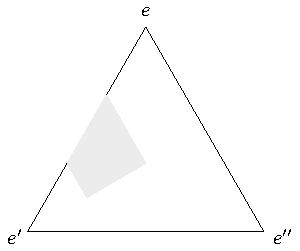
\includegraphics[width=0.32\textwidth]{triangle.pdf}
\vspace{7pt}
\caption{Every point in the above equilateral triangle of height one can be identified with a distribution $\Pr(E\newmid g)$ on $\{e,e',e''\}$, by letting $\Pr(e\newmid g)$ be equal to the perpendicular distance from that point to the edge that opposes the corner that corresponds to $e$, and similarly for $\Pr(e'\newmid g)$ and $\Pr(e''\newmid g)$.
In this way, the grey area depicts the distributions in the credal set 
$\credal(E\newmid g)$ of Equation~\eqref{eq:ternarycredal}.}
\label{fig:ternarycredal}
\end{center}
\end{figure}

If all the local credal sets are precise, a credal network is exactly the same as a Bayesian network.
However, if some of the credal sets $\credal(V\newmid\vbpi)$ are imprecise, then since the local distributions $\Pr(V\newmid\vbpi)$ are only known to belong to these credal sets, they do not determine a unique Bayesian network. Therefore, in general, a credal network corresponds to a set of Bayesian networks $\mathbb{B}$, defined by\footnote{There are also other ways in which the local credal sets of a credal network can be combined to form a global model, depending on the type of credal network that is considered~\cite{Cozman:2000ug}; our definition corresponds to what is called a credal network under complete independence. Our results also apply to credal networks under strong independence, which replace $\mathbb{B}$ by its convex hull, but not to credal networks under epistemic irrelevance~\cite{de2015credal,DeBock:2014bv,deCooman:2010gd} or epistemic independence~\cite{deCampos:2007kg}. 
}
\begin{equation*}
\mathcal{B}\in\mathbb{B}
~
\Leftrightarrow
~
(\forall V\!\in{\bf V})\,
(\forall \vbpi\in\vpi)~
\Pr(V\newmid\vbpi)\in\credal(V\newmid\vbpi).
\end{equation*}
If all the local credal sets are precise, the set $\mathbb{B}$ consists of a single Bayesian network.

An important computational problem in credal networks consists in computing tight lower and upper bounds on the probabilities that correspond to the Bayesian networks $\mathcal{B}$ in $\mathbb{B}$, which are called lower and upper probabilities.
In particular, we consider the problem of computing tight lower and upper bounds on probabilities of the form $\Pr(\hyp\newmid\ev)$, defined by 
\begin{equation}\label{eq:impreciseinferences}
\underline{\Pr}(\hyp \newmid \ev)
\coloneqq
\min_{\mathcal{B}\in\mathbb{B}}
\,
\Pr(\hyp \newmid \ev)
\text{~~\,and\,~~}
\overline{\Pr}(\hyp \newmid \ev)
\coloneqq
\max_{\mathcal{B}\in\mathbb{B}}\,
\Pr(\hyp \newmid \ev).
\end{equation}
\noindent In order for these definitions to make sense, we require that $\Pr(\ev)$ is strictly positive for all $\mathcal{B}\in\mathbb{B}$.\footnote{For a detailed discussion on how to define $\underline{\Pr}(\hyp \newmid \ev)$ and $\overline{\Pr}(\hyp \newmid \ev)$ if $\Pr(\ev)$ is zero for some---but not all---$\mathcal{B}$ in $\mathbb{B}$, see Reference~\cite{DeBock20151}.}

Computing the lower and upper probabilities in Equation~\eqref{eq:impreciseinferences} consists in optimising $\Pr(\hyp\newmid\ev)$, which is a fraction of two multilinear functions of the network's parameters, under the constraint that each of the local distributions $\Pr(V\newmid\vbpi)$ belongs to its credal set $\credal(V\newmid\vbpi)$. Obtaining the exact solution is only possible in special cases~\cite{Fagiuoli:1998ft,Maua:2014ti} or for networks that are sufficiently small. Therefore, applied work on credal networks often resorts to approximate algorithms; see Reference~\cite{Antonucci:2014ty} for a recent overview.

Most of the existing algorithms exploit the fact that for the purposes of computing $\underline{\Pr}(\hyp\newmid\ev)$ or $\overline{\Pr}(\hyp\newmid\ev)$, the---closed and convex---credal sets $\credal(V\newmid\vbpi)$ can be replaced by their set of extreme points\footnote{An extreme point of a set is a point that cannot be written as a proper convex combination of two other points of that set. If a set is a closed and convex subset of a finite-dimensional space, then by Minkowski's finite-dimensional version of the Krein-Milman theorem, it is the convex hull of its extreme points.} $\mathrm{ext}(\credal(V\newmid\vbpi))$~\cite{Fagiuoli:1998ft}:
\begin{equation*}
\underline{\Pr}(\hyp \newmid \ev)
=
\min_{\mathcal{B}\in\mathbb{B}_{\mathrm{ext}}}
\,
\Pr(\hyp \newmid \ev)
\text{~~\,and\,~~}
\overline{\Pr}(\hyp \newmid \ev)
=
\max_{\mathcal{B}\in\mathbb{B}_{\mathrm{ext}}}\,
\Pr(\hyp \newmid \ev),
\end{equation*}
where $\mathbb{B}_{\mathrm{ext}}$ is the set of Bayesian networks in $\mathbb{B}$ whose local distributions $\Pr(V\newmid\vbpi)$ take values in $\mathrm{ext}(\credal(V\newmid\vbpi))$, defined by
\begin{equation*}
\mathcal{B}\in\mathbb{B}_{\mathrm{ext}}
~
\Leftrightarrow
~
(\forall V\!\in{\bf V})\,
(\forall \vbpi\in\vpi)~
\Pr(V\newmid\vbpi)\in\mathrm{ext}
\left(\credal(V\newmid\vbpi)\right).
\end{equation*}

The reason why this is useful is because in practice, credal sets are usually~\emph{finitely generated}, meaning that they are defined by means of a finite number of linear constraints, or equivalently, that they have a finite number of extreme points. For example, the credal set $\credal(G)$ of Equation~\eqref{eq:binarycredal} has two extreme points, which are characterised by $\Pr(g)=\nicefrac{1}{3}$ and $\Pr(g)=\nicefrac{2}{3}$, respectively. Similarly, the credal set $\credal(E\newmid g)$ in Figure~\ref{fig:ternarycredal} has four extreme points $\Pr(E\newmid g)=(\Pr(e\newmid g),\Pr(e'\newmid g),\Pr(e''\newmid g))$:
\begin{equation}\label{eq:fourextremepoints}
(\frac{1}{3},\frac{1}{3},\frac{1}{3}),~~
(\frac{2}{3},\frac{1}{3},0),~~
(\frac{1}{3},\frac{2}{3},0)~~\text{and}~~
(\frac{1}{6},\frac{2}{3},\frac{1}{6}).
\end{equation}
If all the local credal sets are finitely generated, $\mathbb{B}_{\mathrm{ext}}$ is finite, and computing lower and upper probabilities is then a combinatoric optimisation problem, the size of which is exponential in the number of local credal sets that are imprecise. 

\subsection{Removing credal sets}

{\color{red}*** This is the imprecise counterpart to the constant effect section in the precise part of the paper. By d-separatation, removal of barren nodes, and evidence absorbtion, we can shrink the size of the network (this is all known, it's just a recap to contrast it with the next section) ***}

\subsection{Reducing imprecise credal sets to precise ones}\label{sec:credal:reducetosingletons}

{\color{red}  *** Type 0 will disappear here, since it is part of the previous section ***}

As we will now show, in many cases, we can use the sensitivity properties of Section~\ref{sec:bayesian:guaranteedeffects} to reduce the computational complexity of inference in credal networks.

Basically, the idea is that, for the purposes of computing $\underline{\Pr}(\hyp\newmid\ev)$ or $\overline{\Pr}(\hyp\newmid\ev)$, some of the local credal sets of a credal network can be replaced by a singleton, that is, some imprecise local credal sets can be replaced by precise ones, without changing the result of the inference. In this way, the size of the combinatoric optimisation problem that needs to be solved can be reduced in advance, as a preprocessing step, before applying an inference algorithm of choice. 

We introduce four types of local credal sets for which this is the case. Their definitions are completely analogous to the local distribution types that were defined in Section~\ref{sec:bayesian:distributiontypes}. For example, a local credal set $\credal(V\newmid\vbpi)$ is of Type 0 if and only if its distributions are of Type 0, and similarly for credal sets that are of type I, II or III.

\begin{defi}[Local credal set types]\label{def:credaltypes}
Consider a credal network ${\mathbb B}$ and a lower or upper probability of interest $\underline{\Pr}(\hyp\newmid\ev)$ or $\overline{\Pr}(\hyp\newmid\ev)$. A local credal set $\credal(V\newmid \vbpi)$ is then said to be of\\[4pt]
\begin{tabular}{l l}
{\bf Type 0} & if\/ $\vbpi\nsim\ev$\emph{;}\\
{\bf Type I} & if\/ $\vbpi\sim\ev$, $V\in \evs\restr$~~and $\vbpi\sim\hyp$\emph{;}\\
{\bf Type II} & if\/ $\vbpi\sim\ev$, $V\in \evs$ and $\vbpi\nsim\hyp$\emph{;}\\
{\bf Type III} & if\/ $\vbpi\sim\ev$, $\vbpi\sim\hyp$, $V\in \hyps\restr$~~and $\vert V\vert =2$\emph{.}
\end{tabular}
\end{defi}

Since the elements of a credal set $\credal(V\newmid \vbpi)$ of Type 0 are distributions of Type 0, it follows from Proposition~\ref{constant} that this credal set is of no influence to the inference at hand. The following result is an immediate consequence of this fact.

\begin{prop}\label{credalType0}
Consider a credal network ${\mathbb B}$ and a lower or upper probability of interest $\underline{\Pr}(\hyp\newmid\ev)$ or $\overline{\Pr}(\hyp\newmid\ev)$. Then replacing a credal set $\credal(V\newmid \vbpi)$ of\, \emph{Type 0} with a singleton~$\credal'(V\newmid \vbpi)\coloneqq\{\Pr(V\newmid\vbpi)\}$ that consists of an arbitrary probability mass function $\Pr(V\newmid\vbpi)$ on $V$ will not change the result of the inference.
\end{prop}
\noindent
Note that $\Pr(V\newmid\vbpi)$ is not required to be an element of $\credal(V\newmid \vbpi)$, and that it can therefore be chosen as simple as possible.

As we are about to show, similar results can also be obtained for credal sets of Type I, II and III. However, in those cases, the distribution $\Pr(V\newmid\vbpi)$ can no longer be chosen arbitrarily. We start with credal sets of Type I or II.

Since a distribution in a credal set of Type I or II is itself of Type I or II,  we infer from the discussion in Section~\ref{sec:bayesian:distributiontypes} that, for the purposes of computing $\Pr(\hyp\newmid\ev)$, the only part of this distribution that is relevant is the parameter $\Pr(v\newmid \vbpi)$, with $v$ the unique instantiation of $V$ that is compatible with $\ev$. Furthermore, because of the monotone effect of changing this parameter---see Theorem~\ref{theo}---we know that the minimum and maximum value of $\Pr(\hyp\newmid\ev)$ will be obtained by a Bayesian network $\mathcal{B}\in\mathbb{B}_{\mathrm{ext}}$ for which the parameter $\Pr(v\newmid\vbpi)$ is minimal or maximal, in the sense that it is equal to the local lower probability
\begin{equation*}
\underline{\Pr}(v\newmid\vbpi)\coloneqq\min_{\Pr(V\newmid\vbpi)\in\credal(V\newmid\vbpi)}\Pr(v\newmid\vbpi)
\end{equation*}
or the local upper probability
\begin{equation*}
\overline{\Pr}(v\newmid\vbpi)\coloneqq\max_{\Pr(V\newmid\vbpi)\in\credal(V\newmid\vbpi)}\Pr(v\newmid\vbpi),
\end{equation*}
and we can predict in advance which of these two extreme values it will be. Combined, these two observations allow us to replace the (possibly imprecise) credal set $\credal(V\newmid \vbpi)$ with a precise one. The following proposition makes this explicit.

{\color{red}*** after this result, I intend to strenghten the result even more by combining it with the fact that the credal set can be taken to be binary (as Antonucci already showed in a paper of his), provided that we already did the d-sep, barren and evidence absorbtion (which implies that all evidence are leafs), thereby proving that the credal sets of the evidence leafs can be replaced by precise binary distributions ***}

\begin{prop}\label{prop:credalTypeIorII}
Consider a credal network ${\mathbb B}$ and a lower or upper probability of interest $\underline{\Pr}(\hyp\newmid\ev)$ or $\overline{\Pr}(\hyp\newmid\ev)$. A credal set $\credal(V\newmid \vbpi)$ of\/ Type I or II can then be replaced with a singleton~$\credal'(V\newmid \vbpi)\coloneqq\{\Pr(V\newmid\vbpi)\}$, without changing the result of the inference. If we let $v$ be the unique value of\/ $V$ that is compatible with $\ev$, then for $\underline{\Pr}(\hyp\newmid\ev)$, $\Pr(V\newmid\vbpi)$ can be any probability mass function on $V$ such that
\begin{equation*}
\Pr(v\newmid\vbpi)
=
\begin{cases}
\underline{\Pr}(v\newmid\vbpi)
& \text{if\/ $\credal(V\newmid\vbpi)$ is of Type I\emph{;}}\\
\overline{\Pr}(v\newmid\vbpi)
& \text{if\/ $\credal(V\newmid\vbpi)$ is of Type II\emph{,}}
\end{cases}
\end{equation*}
and for $\overline{\Pr}(\hyp\newmid\ev)$, $\Pr(V\newmid\vbpi)$ can be any probability mass function on $V$ such that
\vspace{-4pt}
\begin{equation*}
\Pr(v\newmid\vbpi)
=
\begin{cases}
\overline{\Pr}(v\newmid\vbpi)
& \text{if\/ $\credal(V\newmid\vbpi)$ is of Type I\emph{;}}\\
\underline{\Pr}(v\newmid\vbpi)
& \text{if\/ $\credal(V\newmid\vbpi)$ is of Type II\emph{.}}
\end{cases}
\end{equation*}
\end{prop}
{\bf Proof.}
We only prove the result for $\underline{\Pr}(\hyp\newmid\ev)$; the proof for $\overline{\Pr}(\hyp\newmid\ev)$ is completely analogous.

If the local credal set $\credal(V\newmid \vbpi)$ is of Type I, then because of Theorem~\ref{theo}, the minimum value of $\Pr(\hyp\newmid\ev)$ is obtained for a local distribution $\Pr(V\newmid\vbpi)$ of which the parameter $\Pr(v\newmid\vbpi)$ is minimal---equal to $\underline{\Pr}(v\newmid\vbpi)$. Furthermore, due to Proposition~\ref{constant}, the other parameters of this local distribution are irrelevant. Hence, for the purposes of computing $\underline{\Pr}(\hyp\newmid\ev)$, $\credal(V\newmid \vbpi)$ can be replaced by a precise credal set~$\credal'(V\newmid \vbpi)\coloneqq\{\Pr(V\newmid\vbpi)\}$ that consists of a single distribution $\Pr(V\newmid\vbpi)$ on $V$, with $\Pr(v\newmid\vbpi)=\underline{\Pr}(v\newmid\vbpi)$. 
If the local credal set $\credal(V\newmid \vbpi)$ is of Type II, it follows from Theorem~\ref{theo} that the minimum value of $\Pr(\hyp\newmid\ev)$ is obtained for a local distribution $\Pr(V\newmid\vbpi)$ of which the parameter $\Pr(v\newmid\vbpi)$ is maximal---equal to $\overline{\Pr}(v\newmid\vbpi)$---and therefore, $\credal(V\newmid \vbpi)$ can again be replaced by a singleton that consists of a single distribution $\Pr(V\newmid\vbpi)$, now with $\Pr(v\newmid\vbpi)=\overline{\Pr}(v\newmid\vbpi)$.
\hfill$\Box$

\bigskip

\noindent
Note that $\Pr(V\newmid\vbpi)$ is again not required to be an element of $\credal(V\newmid \vbpi)$, which allows us to choose it as simple as possible.

Consider for example the network in Figure~\ref{fig-vbMAP-TC}, and assume that we want to compute $\underline{\Pr}(ghk\newmid ef)$. The local credal set $\credal(E\newmid g)$---defined in Equation~\eqref{eq:ternarycredal} and depicted in Figure~\ref{fig:ternarycredal}---is then of Type I and can therefore be replaced by a singleton $\credal'(E\newmid g)=\{\Pr(E\newmid g)\}$, where $\Pr(E\newmid g)$ can be any probability mass function on $\{e,e',e''\}$ such that
\begin{equation*}
\Pr(e\newmid g)\coloneqq\underline{\Pr}(e\newmid g)=\frac{1}{6}.
\end{equation*}
The values of $\Pr(e'\newmid g)$ and $\Pr(e''\newmid g)$ are of no importance. If we want $\Pr(E\newmid g)$ to belong to $\credal(E\newmid g)$, then the only possible choice is $\Pr(e'\newmid g)=\nicefrac{2}{3}$ and $\Pr(e''\newmid g)=\nicefrac{1}{6}$, which corresponds to one of the extreme points in Equation~\eqref{eq:fourextremepoints}. However, this is not necessary. For example, choosing $\Pr(e'\newmid g)=0$ and $\Pr(e''\newmid g)=\nicefrac{5}{6}$ works equally well.

Finally, for local credal sets that are of Type III, we obtain a result that is very similar to that of Proposition~\ref{prop:credalTypeIorII}.

\begin{prop}\label{prop:credalTypeIII}
Consider a credal network ${\mathbb B}$ and a lower or upper probability of interest $\underline{\Pr}(\hyp\newmid\ev)$ or $\overline{\Pr}(\hyp\newmid\ev)$. A credal set $\credal(V\newmid \vbpi)$ of\/ Type III can then be replaced with a singleton~$\credal'(V\newmid \vbpi)\coloneqq\{\Pr(V\newmid\vbpi)\}$, without changing the result of the inference. For $\underline{\Pr}(\hyp\newmid\ev)$, $\Pr(V\newmid\vbpi)$ is defined by
\begin{equation}\label{eq:singleton:typeIII:lower}
\Pr(v\newmid\vbpi)
\coloneqq
\begin{cases}
\underline{\Pr}(v\newmid\vbpi)
& \text{if\/ $v\sim\hyp$\emph{;}}\\
\overline{\Pr}(v\newmid\vbpi)
& \text{if\/ $v\nsim\hyp$\emph{,}}
\end{cases}
\end{equation}
and for $\overline{\Pr}(\hyp\newmid\ev)$, $\Pr(V\newmid\vbpi)$ is defined by
\begin{equation*}
\Pr(v\newmid\vbpi)
\coloneqq
\begin{cases}
\overline{\Pr}(v\newmid\vbpi)
& \text{if\/ $v\sim\hyp$\emph{;}}\\
\underline{\Pr}(v\newmid\vbpi)
& \text{if\/ $v\nsim\hyp$\emph{.}}
\end{cases}
\end{equation*}
\end{prop}
{\bf Proof.}
We only prove the result for $\underline{\Pr}(\hyp\newmid\ev)$; the proof for $\overline{\Pr}(\hyp\newmid\ev)$ is completely analogous.

Let $v$ be the unique value of $V$ that is compatible with $\hyp$.
If the local credal set $\credal(V\newmid \vbpi)$ is of Type III, then because of Theorem~\ref{theo}, the minimum value of $\Pr(\hyp\newmid\ev)$ is obtained for a local distribution $\Pr(V\newmid\vbpi)$ of which the parameter $\Pr(v\newmid\vbpi)$ is minimal---equal to $\underline{\Pr}(v\newmid\vbpi)$---and the parameter $\Pr(\overline{v}\newmid\vbpi)$ is maximal. The unique distribution for which this is the case is given by Equation~\eqref{eq:singleton:typeIII:lower}. Hence, for the purposes of computing $\underline{\Pr}(\hyp\newmid\ev)$, $\credal(V\newmid \vbpi)$ can be replaced by the singleton~$\credal'(V\newmid \vbpi)\coloneqq\{\Pr(V\newmid\vbpi)\}$.
\hfill$\Box$

\bigskip

\noindent
Note that in this case, $\Pr(V\newmid\vbpi)$ is unique and belongs to $\credal(V\newmid \vbpi)$.

For example, if we again consider the network in Figure~\ref{fig-vbMAP-TC}, and revisit the problem of computing $\underline{\Pr}(ghk\newmid ef)$, then the local credal set $\credal(G)$---defined in Equation~\eqref{eq:binarycredal}---is of Type III and can therefore be replaced by a singleton $\credal'(G)=\{\Pr(G)\}$, with
\begin{equation*}
\Pr(g)\coloneqq\underline{\Pr}(g)=\nicefrac{1}{3}
\text{ and }\Pr(g)\coloneqq\overline{\Pr}(g)=\nicefrac{2}{3}.
\end{equation*}

In our example, in total, eight out of the fifteen credal sets of the credal network in Figure~\ref{fig-vbMAP-TC} can be replaced by a singleton, whereas other preprocessing techniques---such as the removal of barren or d-separated nodes---are not able to simplify the problem.


\subsection{Special cases and examples}\label{sec:credal:specialcase}

Since a local credal set is of a given type if and only if its elements are, the special cases that were discussed in Section~\ref{sec:bayesian:specialcase} carry over to credal networks. For example, for a credal network classifier with full evidence, the credal sets that correspond to the evidence variables are all of Type 0, I or II, and therefore, they can be replaced by singletons. It is essentially this feature that allows for tractable computations in basic credal classifiers such as the naive credal classifier \cite{Zaffalon:2002bn} and the tree-augmented naive classifier~\cite{Zaffalon:2003gq}. In fact, many of the formulas in References~\cite{Zaffalon:2002bn} and~\cite{Zaffalon:2003gq} can be shown to follow from our results.

{\color{red} *** I will explicitly derive the formulas in the references above. First for the general special case of a classifier with full evidence (this consists of first moving to the Markov blanket by dropping credal sets, and then turning the remaining evidence credal sets into precise (binary!) ones), and then for the specific classifiers they consider, and also for HMMs (if only the observations are imprecise, then this is very efficient!)! For the non-binary case, this will lead to the same substitutions they do.}

In the special case where we do not only have full evidence, but also know that each of the hypothesis variables $V\in\hyps$ is binary and has no parents in $\hyps$, then all the local credal sets of the credal network can be classified as one of the four types in Definition~\ref{def:credaltypes}. 
This has far-reaching consequences: in this case, due to the results in the previous section, it follows that for the purpose of computing $\underline{\Pr}(\hyp\newmid\ev)$ or $\overline{\Pr}(\hyp\newmid\ev)$, all the local credal sets can be replaced by singletons, without changing the result of the inference.
Hence, in this case, computing $\underline{\Pr}(\hyp\newmid\ev)$ or $\overline{\Pr}(\hyp\newmid\ev)$ reduces to the problem of computing $\Pr(\hyp\newmid\ev)$ in a specific Bayesian network, the parameters of which can easily be determined by means of the methods in Section~\ref{sec:credal:reducetosingletons}.

{\color{red}*** For the binary case, the expressions above will now lead to closed-form expressions, which I will provide. ***}

For example, in this special case, for the purpose of computing $\underline{\Pr}(\hyp\newmid\ev)$, the local credal sets of a credal network can be replaced by precise distributions ${\Pr}_{\bullet}(V\newmid\vbpi)$, the parameters of which are defined by
\vspace{-6pt}
\begin{equation}\label{eq:explicitsingletonslowercase}
{\Pr}_{\bullet}(v\newmid\vbpi)
\coloneqq
\begin{cases}
\underline{\Pr}(v\newmid\vbpi) &\text{if~$V\in\hyps$ and $v\sim\hyp$}\\
\overline{\Pr}(v\newmid\vbpi) &\text{if~$V\in\hyps$ and $v\nsim\hyp$}\\
\underline{\Pr}(v\newmid\vbpi) &\text{if~$V\in\evs$, $v\sim\ev$ and $\vbpi\sim\hyp$}\\
\overline{\Pr}(v\newmid\vbpi) &\text{if~$V\in\evs$, $v\sim\ev$ and $\vbpi\nsim\hyp$}\\
$...$ &\text{if~$V\in\evs$ and $v\nsim\ev$}
\end{cases}
\vspace{6pt}
\end{equation}
This definition does not distinguish between the cases $\vbpi\sim\ev$ and $\vbpi\nsim\ev$ because we know from Proposition~\ref{credalType0} that a parameter for which $\vbpi\nsim\ev$ does not effect the result of the inference anyway. Similarly, the definition for the case with $V\in\evs$ and $v\nsim\ev$ is not provided because we know from Proposition~\ref{prop:credalTypeIorII} that these parameters do not influence the result of the inference either.

As an immediate consequence, for this special case, we obtain the following expression:
\begin{align*}
\underline{\Pr}(\hyp\newmid\ev)
=\frac
{\prod_{V\in{\bf V}}{\Pr}_{\bullet}(v\newmid\vbpi)\giv{v\vbpi\sim \hyp\ev}}
{\sum_{\hyp^*\in\hyps}\prod_{V\in{\bf V}}{\Pr}_{\bullet}(v\newmid\vbpi)\giv{v\vbpi\sim \hyp^*\ev}}%\\
\end{align*}
Furthermore, by removing the parameters ${\Pr}_{\bullet}(v\newmid\vbpi)$ for which $V$ and its parents $\vpi$ belong to $\evs$---since these are common factors of the numerator and denominator---and then explicitly applying Equation~\eqref{eq:explicitsingletonslowercase} to the numerator, this expression can be simplified even more:
\vspace{-6pt}
\begin{equation*}
\underline{\Pr}(\hyp\newmid\ev)
=
\frac
{\prod_{V\in{\bf K}}\underline{\Pr}(v\newmid\vbpi)\giv{v\vbpi\sim \hyp\ev}}
{\sum_{\hyp^*\in\hyps}\prod_{V\in{\bf K}}{\Pr}_{\bullet}(v\newmid\vbpi)\giv{v\vbpi\sim \hyp^*\ev}}
\vspace{2pt}
\end{equation*}
where ${\bf K}$ is the set of variables that consist of the variables in $\hyps$ and their children variables.

Similar conclusions can be reached for the problem of computing $\overline{\Pr}(\hyp\newmid\ev)$. In the special case of Section~\ref{sec:bayesian:specialcase}, this problem can again be reduced to computing $\Pr(\hyp\newmid\ev)$ in a single Bayesian network. 
However, of course, it might not be the same Bayesian network as the one that is used to compute $\underline{\Pr}(\hyp\newmid\ev)$. In this case, the local credal sets can be replaced by distributions ${\Pr}^{\bullet}(V\newmid\vbpi)$, the parameters of which are defined by
\begin{equation*}
{\Pr}^{\bullet}(v\newmid\vbpi)
\coloneqq
\begin{cases}
\overline{\Pr}(v\newmid\vbpi) &\text{if~$V\in\hyps$ and $v\sim\hyp$}\\
\underline{\Pr}(v\newmid\vbpi) &\text{if~$V\in\hyps$ and $v\nsim\hyp$}\\
\overline{\Pr}(v\newmid\vbpi) &\text{if~$V\in\evs$, $v\sim\ev$ and $\vbpi\sim\hyp$}\\
\underline{\Pr}(v\newmid\vbpi) &\text{if~$V\in\evs$, $v\sim\ev$ and $\vbpi\nsim\hyp$}\\
$...$ &\text{if~$V\in\evs$ and $v\nsim\ev$}
\end{cases}
\vspace{2pt}
\end{equation*}

\section{Experiments}

{\color{red}*** I'll try to conduct some experiments to show how the number of reduced credal sets depends on the inference, the topology, ..., with randomly generated networks and inferences ***}

{\color{red}*** I'll ask Allessandro whether he thinks he can apply our closed-form expressions to run some multilabel classifier experiments with real data ***}

{\color{red}*** We'll add some experiments on how well our methods perform as a preprocessing technique. Existing algorithms focus on cases with a single hypothesis variable though... so the effect might be relatively small. I'll try to run some brute force experiments for more general cases as well... ***}

{\color{red} *** A reviewer of the conference version asked to check the effect on the branch and bound algorithm of Da Rocha and Cozman. I'll check whether this is feasible. If not, I'll just add the algorithm as a reference and leave it as future work ***}

{\color{red}*** Can also help to develop new algorithms (in message passing of polytopes, does it help?) *** Reduce more general topologies to polytrees? ***}

\section{Conclusions and future work}\label{sec:conclusion}

A credal network represents a set of Bayesian networks thereby allowing for imprecisions in its parametrisation. One of the main computational problems in a credal network is the computation of lower and upper probabilities. Given a brute force approach, however, this requires a number of Bayesian network inferences that is exponential in the number of imprecisely specified local probability distributions.

The pruning of all variables irrelevant for a specific problem is a well-known approach to make inference more tractable. In this paper we proposed a different type of preprocessing step. Using Bayesian network sensitivity functions, we proved that for certain categories of parameters, we can predict the qualitative effect of their change on an outcome probability without needing any knowledge of the numerical specification of the network. This result allows for the identification of imprecisely specified local distributions that can be replaced by precisely specified ones, without affecting the outcome of the computation.  Depending on the structure of the network and the specific problem at hand, our preprocessing step can be quite rewarding. We argued, for example, that for some classes of networks, even all imprecisely specified local distributions can be replaced by precise ones. In this case, credal network inference reduces to a single Bayesian network computation.

In future work, we would like to investigate the empirical impact of our preprocessing step on various existing algorithms. Moreover, we would like to use our results as a basis for the design of new algorithms.
For example, we foresee that the algorithm in \cite{Fagiuoli:1998ft} could be extended to more general cases. Finally, we would like to extend our work to other types of inference, such as the computation of lower and upper expectations, choosing the most likely hypothesis, and maximising expected utility.


\subsection*{Acknowledgements}

This research was supported by the Netherlands Organisation for Scientific Research (NWO) and the Fund for Scientific Research -- Flanders (FWO). The authors would also like to thank two anonymous reviewers of a previous conference version, for their generous constructive comments that led to several improvements of this paper.

\bibliographystyle{plain} 
\bibliography{general}

%\appendix

%\section{Proofs}\label{app:proofs}

\end{document}
